%==============================================================
\section{Results}
\label{sec:results}
%==============================================================

This chapter presents the empirical evaluation of four deep learning
architectures for Wi-Fi CSI–based human identification. The analysis is
organised in two phases:

\begin{enumerate}
    \item a four–model benchmark conducted on \textbf{14 November}, where all
    architectures were trained under identical conditions to determine the
    most promising design; and
    \item a DenseNet-only hyperparameter optimisation conducted on
    \textbf{27 November}, where several configurations of the best model were
    explored in depth.
\end{enumerate}

All experiments were tracked using MLflow, ensuring reproducibility and
a fair comparison across models and runs. Performance is primarily measured
using validation accuracy, macro F1-score, and per-class precision/recall
on a validation and a held-out train / test split comprising 2400 CSV Files (if Size 1.94 GB) samples having data of
30 subject classes.

%---------------------------------------------------------------
\subsection{Overall Performance Overview}

Across all experiments, the deep learning models demonstrated strong
capability to discriminate between 30 individuals based solely on their
gait-induced CSI patterns. The best models achieved macro precision,
recall and F1-scores close to $0.98$--$0.99$, indicating that
class-specific performance is uniformly high with no major class being
systematically misclassified. These findings corroborate prior work
on CSI-based HAR and identification, which reported accuracies in the
range of 90--99\,\% using convolutional and recurrent networks
\parencite{zhuravchak2022csihar, csibench2025}.

%==============================================================
\subsection{14 November: Four-Model Comparative Analysis}
\label{subsec:four_model_comparison}
%==============================================================

In the first phase, four architectures were evaluated:

\begin{itemize}
    \item \textbf{CSILSTMNet}: a dual-LSTM baseline operating on CSI and
          metadata sequences.
    \item \textbf{DenseNet1D}: a 1D convolutional DenseNet variant.
    \item \textbf{EfficientNet1D-LSTM}: a hybrid EfficientNet-style 1D CNN
          followed by an LSTM.
    \item \textbf{MobileNetV3-1D-LSTM}: a lightweight MobileNetV3-style 1D CNN
          followed by an LSTM.
\end{itemize}

All models were trained for 150 epochs with a batch size of $8$, learning
rate $1\times 10^{-4}$, Adam optimizer and weight decay
$1\times 10^{-5}$. This controlled setting ensured that architectural
differences, rather than hyperparameters, were the primary driver of
performance differences.

\begin{table}[H]
\centering
\scriptsize
\caption{14 November --- Performance comparison of four deep learning architectures.}
\label{tab:four_model_comparison}
\begin{tabular}{|l|c|c|c|p{4.8cm}|}
\hline
\textbf{Model} &
\textbf{Validation Accuracy} &
\textbf{Macro F1} &
\textbf{Stability} &
\textbf{Remarks} \\ \hline

CSILSTMNet &
0.92 &
0.92 &
Low &
Pure LSTM baseline; no explicit spatial feature extraction, more sensitive to CSI noise and requiring stronger regularisation. \\ \hline

MobileNetV3\_1D\_LSTM &
0.93--0.94 &
0.93 &
Moderate &
Lightweight CNN--LSTM; provides good speed--accuracy trade-off for resource-constrained devices. \\ \hline

EfficientNet1D-LSTM &
0.95--0.96 &
0.95 &
High &
Hybrid EfficientNet-style CNN with LSTM; converges smoothly and generalises well across subjects. \\ \hline

\textbf{DenseNet1D} &
\textbf{0.96} &
\textbf{0.96} &
\textbf{Very High} &
\textbf{Best-performing model; dense connectivity enables strong feature reuse, robust gradient flow and superior discrimination of fine-grained gait patterns.} \\ \hline
\end{tabular}
\end{table}
\begin{figure}[H]
    \centering
    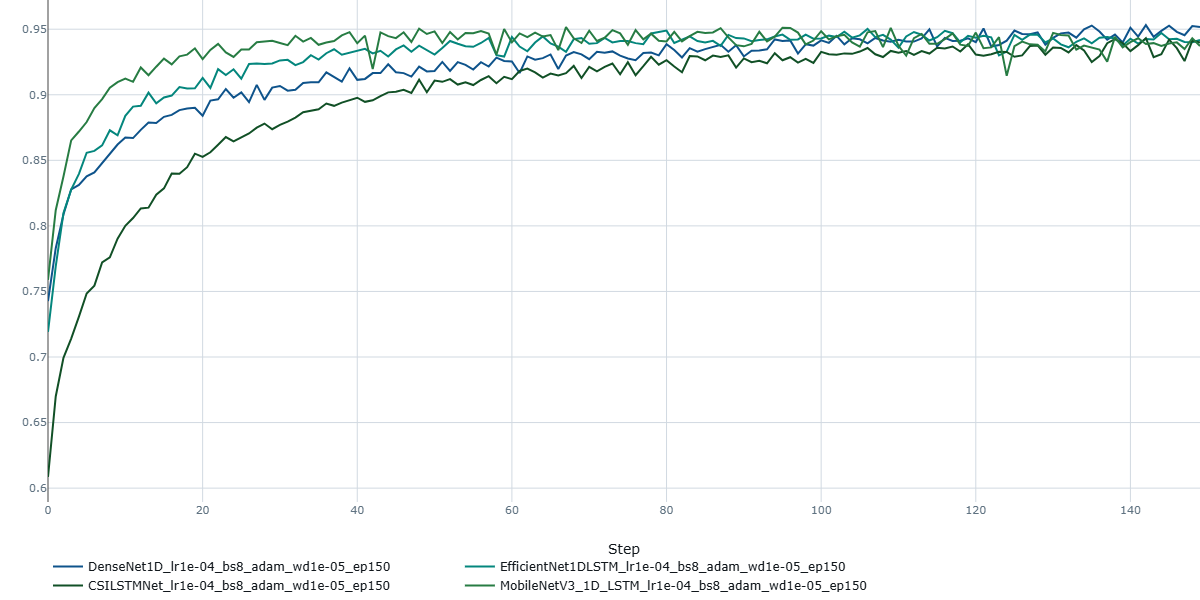
\includegraphics[width=0.7\textwidth]{figures/mlops/Validation Accuracy Curve.png}
    \caption{Validation accuracy comparison of 4 models over epochs using MLFlow}
    \label{fig:mlflow_val_acc1}
\end{figure}
\begin{figure}[H]
    \centering
    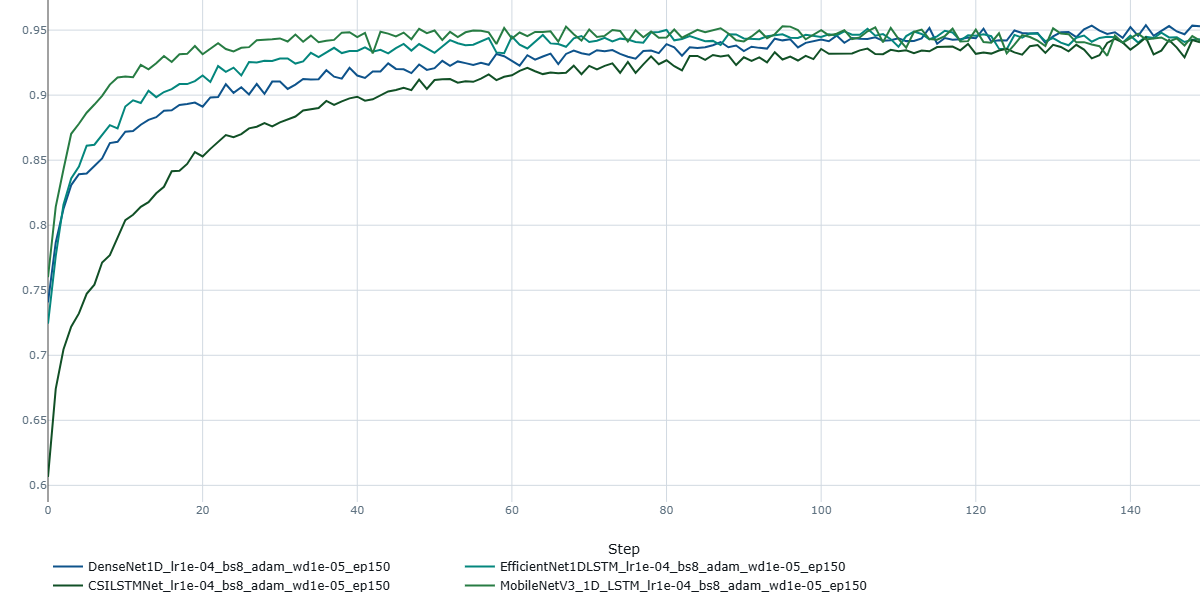
\includegraphics[width=0.7\textwidth]{figures/mlops/Validation Precision Curve.png}
    \caption{Validation precision comparison of 4 models over epochs using MLFlow}
    \label{fig:mlflow_val_prec1}
\end{figure}
\begin{figure}[H]
    \centering
    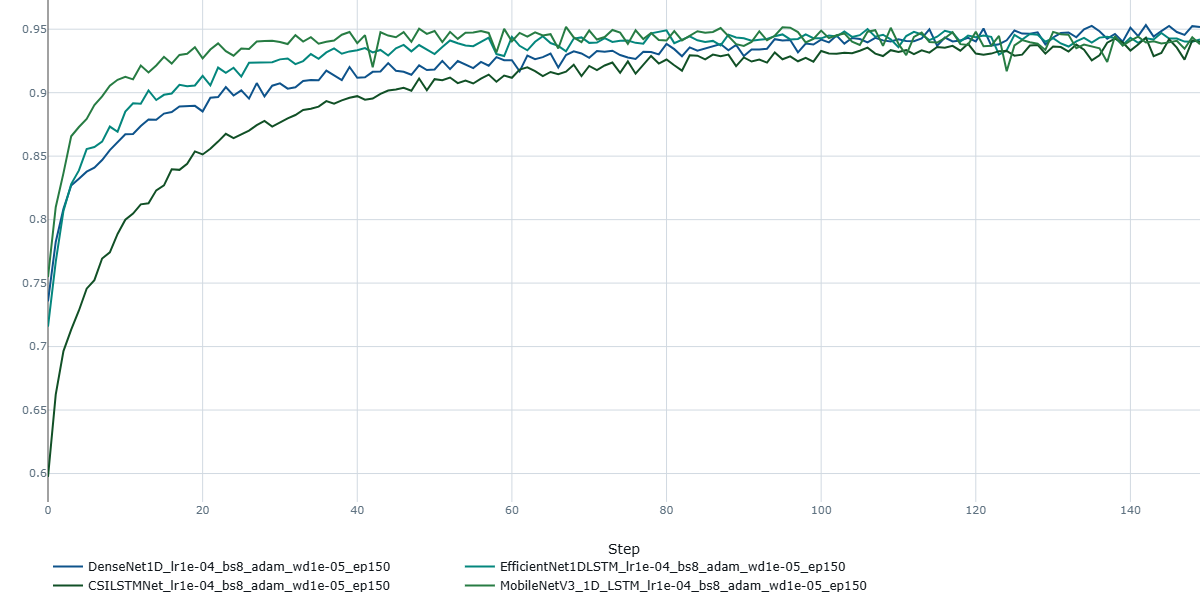
\includegraphics[width=0.7\textwidth]{figures/mlops/Validation F1 Score.png}
    \caption{Validation F1-score comparison of 4 models over epochs using MLFlow}
    \label{fig:mlflow_val_f11}
\end{figure}

The learning curves from the 14 November runs (see
Figures~\ref{fig:csilstm_stats_14nov}--\ref{fig:densenet_stats_14nov}) show
that DenseNet1D and EfficientNet1D-LSTM converge more rapidly and
stably than CSILSTMNet and MobileNetV3-1D-LSTM. DenseNet1D reaches
validation accuracies above $0.94$ within the first 40 epochs and then
continues to improve steadily towards $\approx 0.96$, whereas
CSILSTMNet exhibits higher variance and slower convergence.  

The corresponding confusion matrices
(Figures~\ref{fig:csilstm_cm_14nov}--\ref{fig:densenet_cm_14nov}) display
strong diagonal dominance for all models, with DenseNet1D and
EfficientNet1D-LSTM showing the least off-diagonal mass. Misclassifications
are rare and, when present, usually occur between subjects whose gait
patterns appear highly similar.

\begin{figure}[H]
\centering
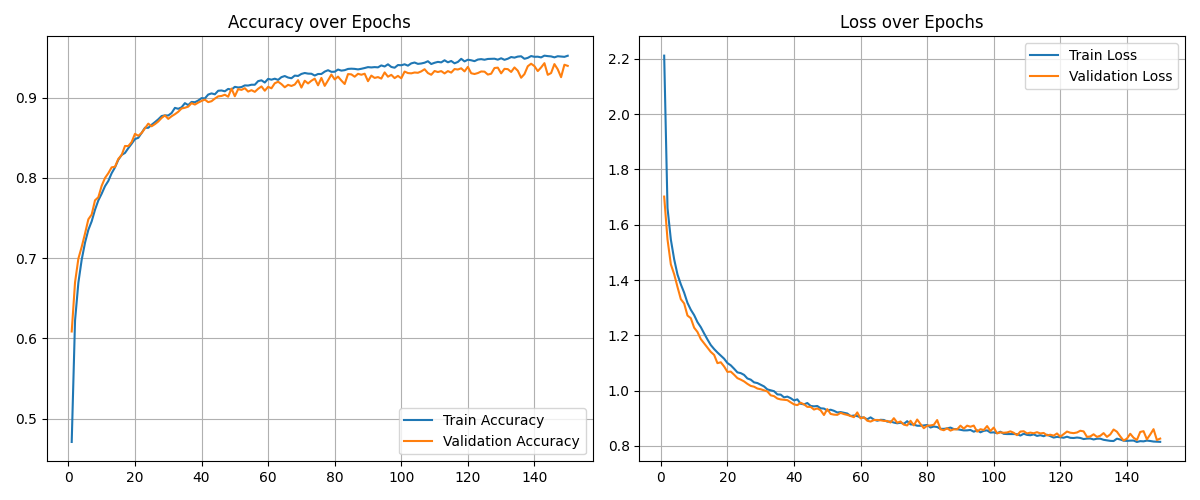
\includegraphics[width=0.9\textwidth]{figures/14nov/CSILSTMNet_lr1e-04_bs8_adam_wd1e-05_ep150_stats.png}
\caption{CSILSTMNet (14 Nov): training and validation accuracy/loss over epochs.}
\label{fig:csilstm_stats_14nov}
\end{figure}

\begin{figure}[H]
\centering
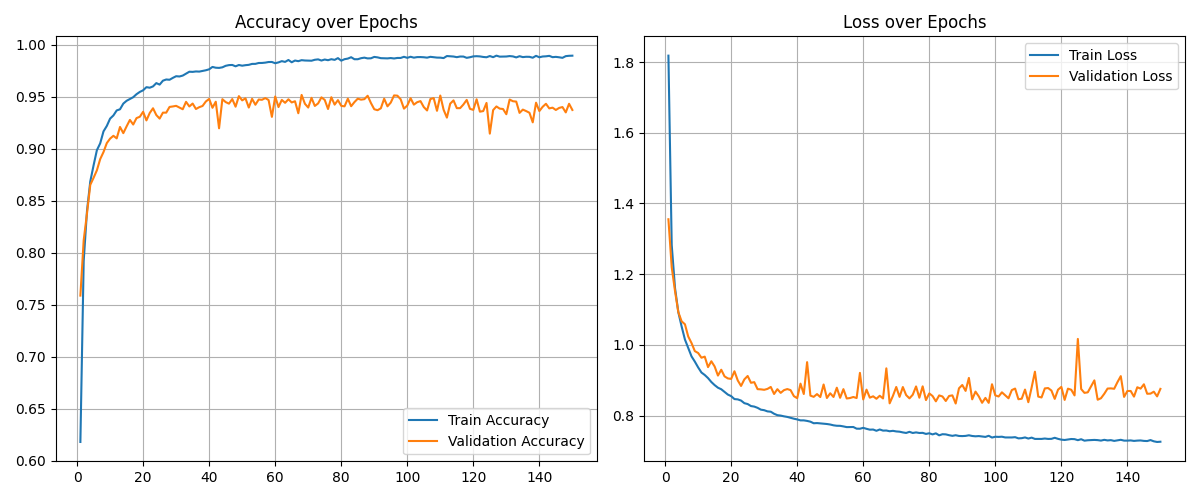
\includegraphics[width=0.9\textwidth]{figures/14nov/MobileNetV3_1D_LSTM_lr1e-04_bs8_adam_wd1e-05_ep150_stats.png}
\caption{MobileNetV3-1D-LSTM (14 Nov): training and validation accuracy/loss over epochs.}
\label{fig:mobnet_stats_14nov}
\end{figure}

\begin{figure}[H]
\centering
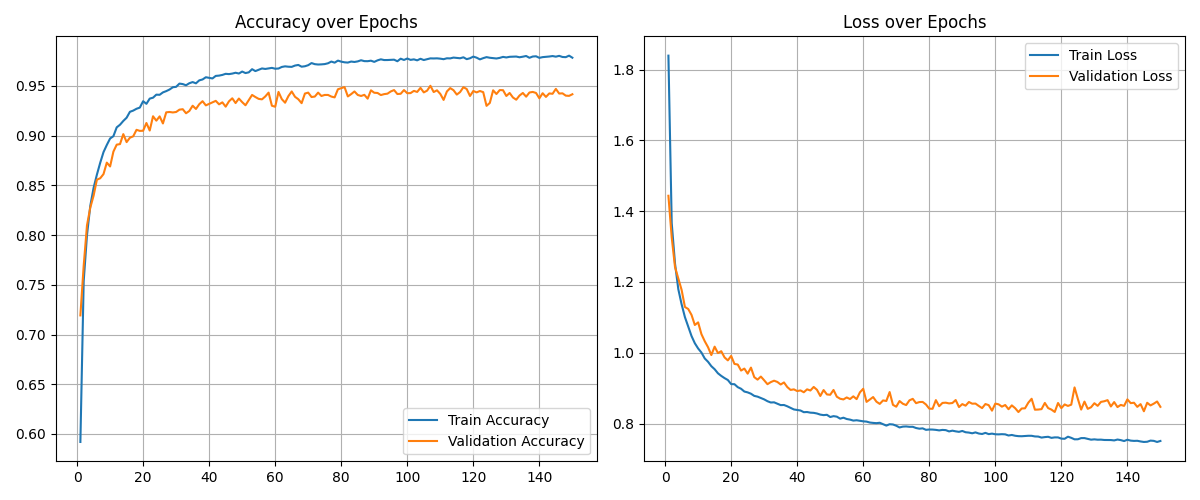
\includegraphics[width=0.9\textwidth]{figures/14nov/EfficientNet1DLSTM_lr1e-04_bs8_adam_wd1e-05_ep150_stats.png}
\caption{EfficientNet1D-LSTM (14 Nov): training and validation accuracy/loss over epochs.}
\label{fig:efficient_stats_14nov}
\end{figure}

\begin{figure}[H]
\centering
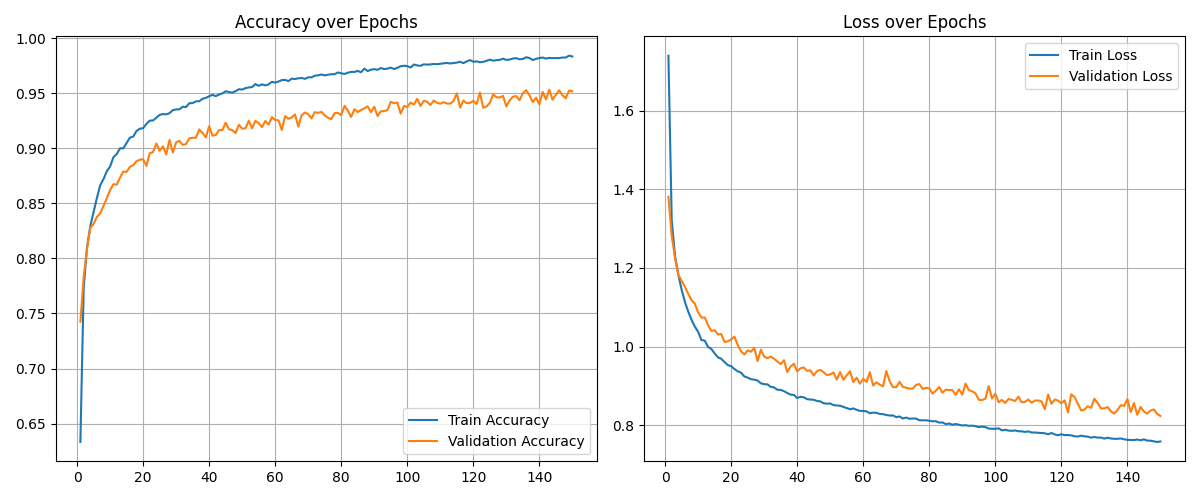
\includegraphics[width=0.9\textwidth]{figures/14nov/DenseNet1D_lr1e-04_bs8_adam_wd1e-05_ep150_stats.png}
\caption{DenseNet1D (14 Nov): training and validation accuracy/loss over epochs.}
\label{fig:densenet_stats_14nov}
\end{figure}

\begin{figure}[H]
\centering
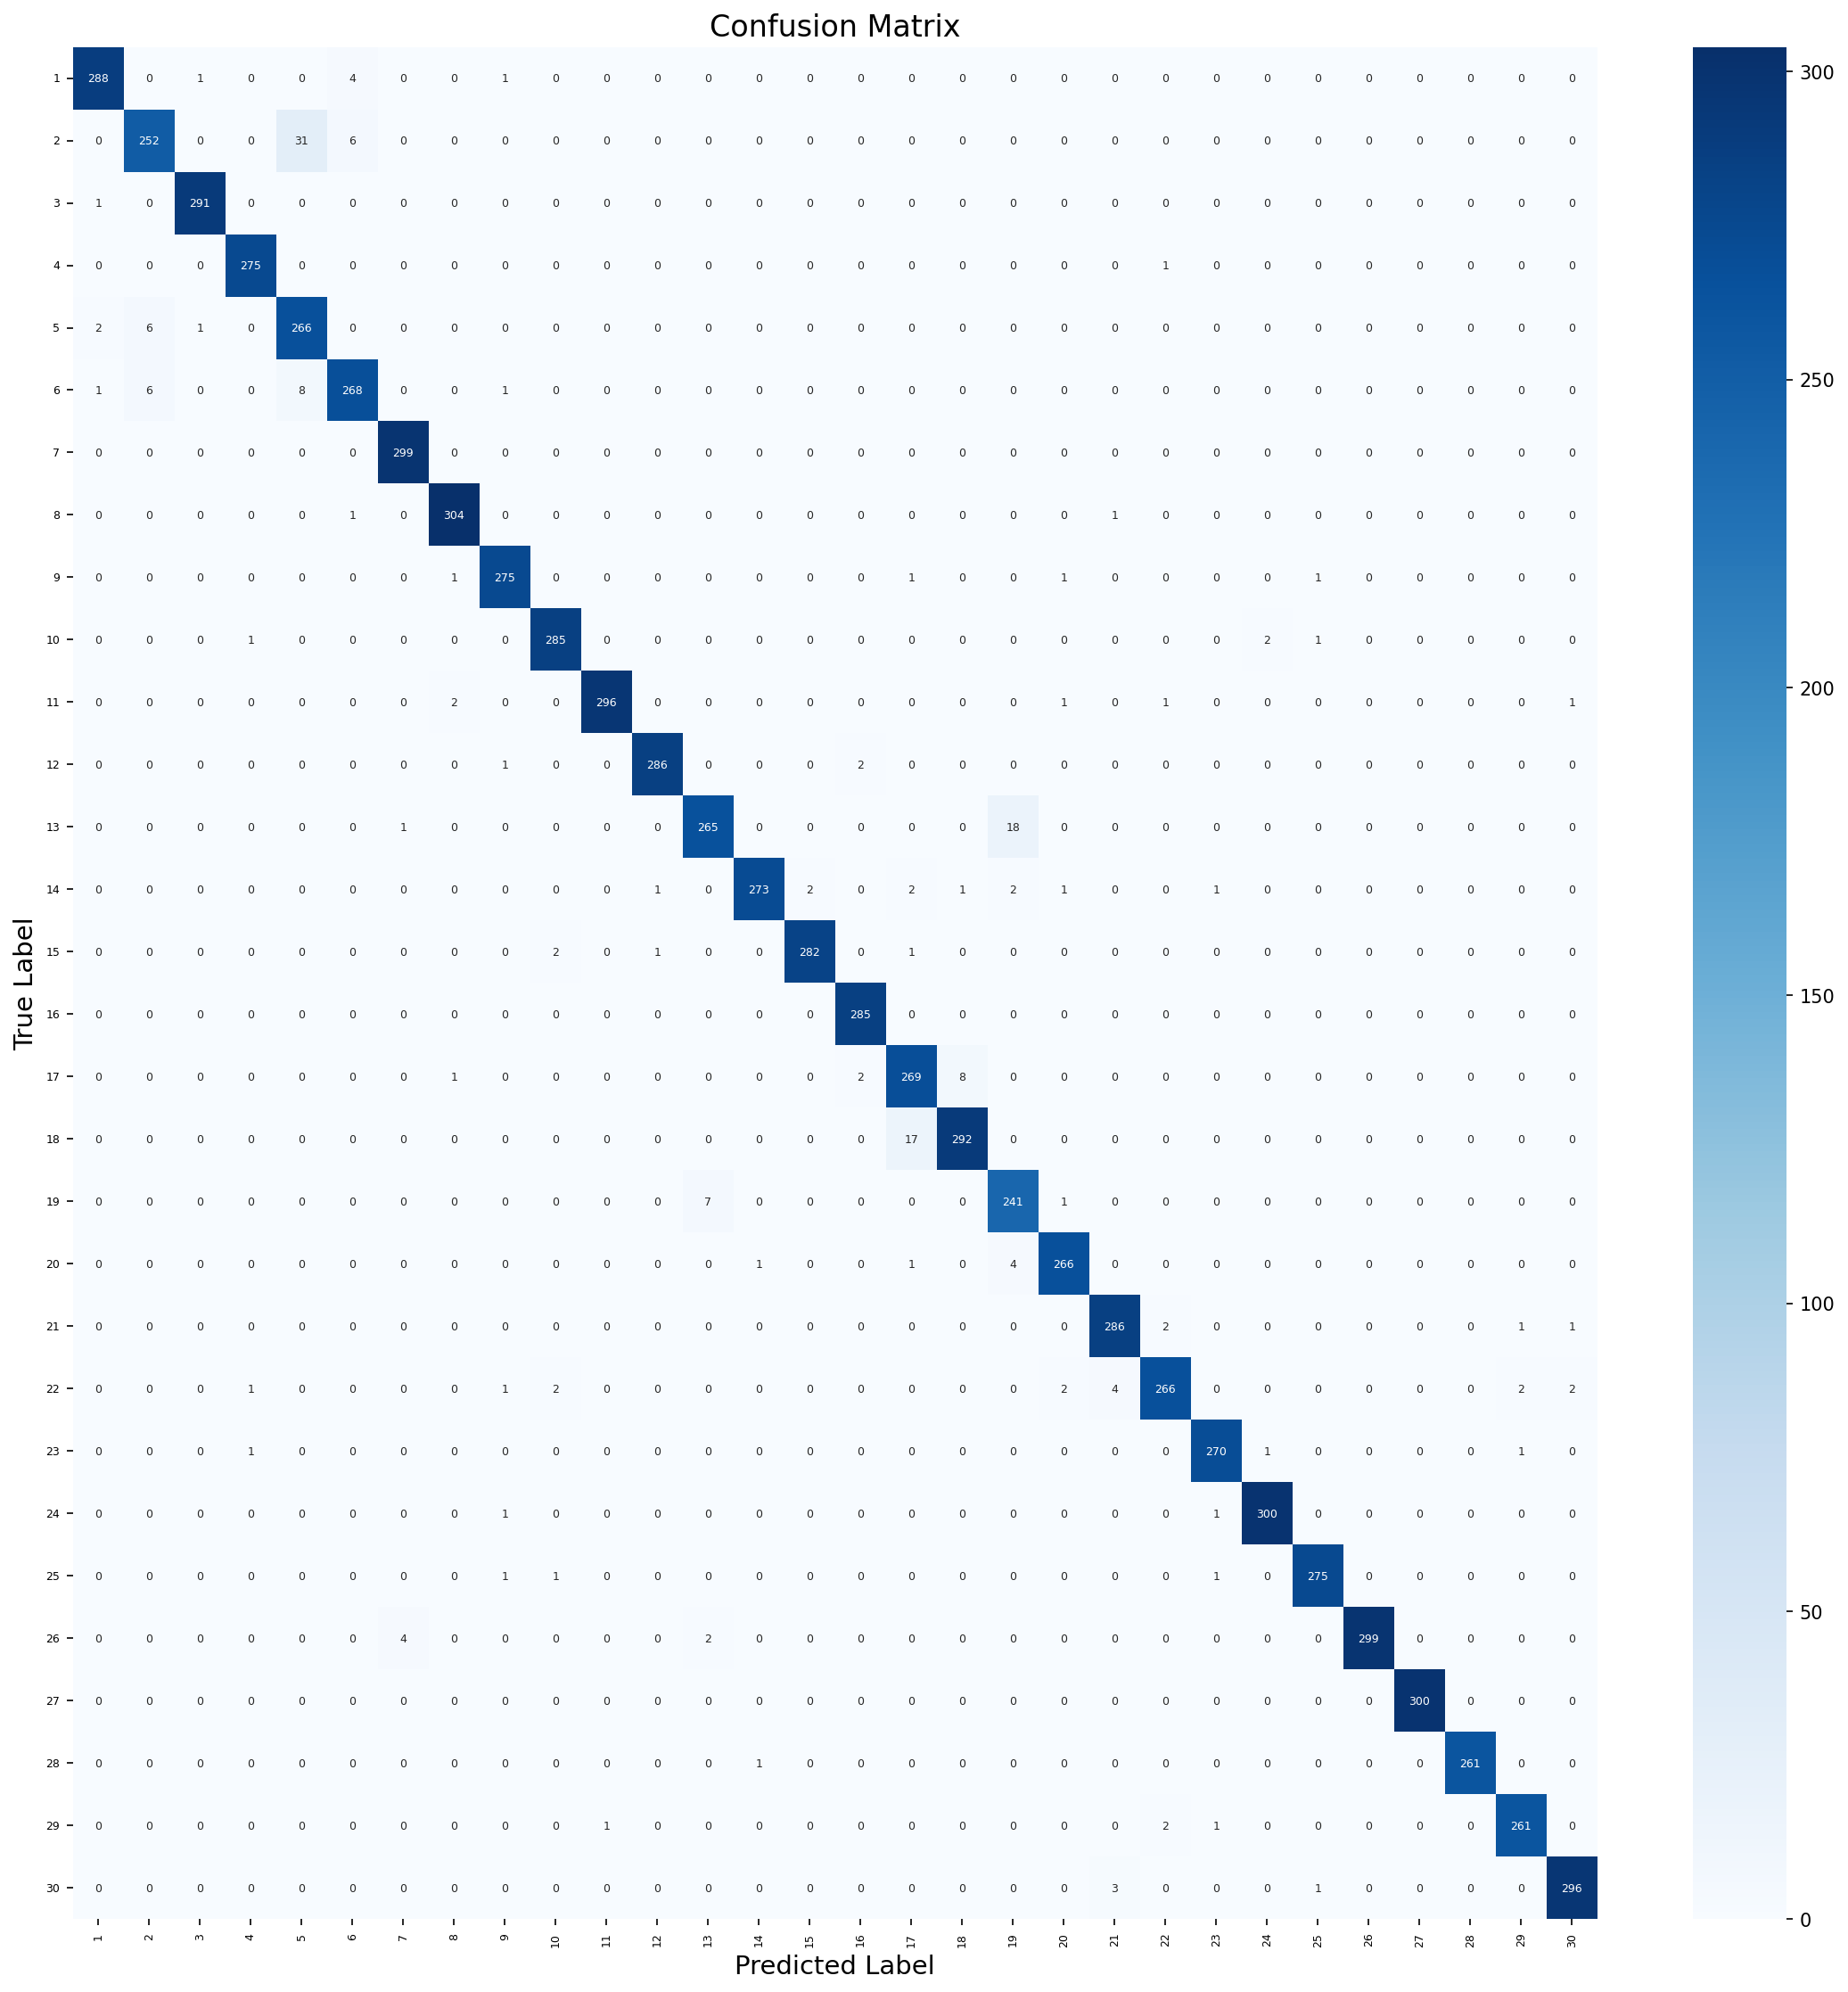
\includegraphics[width=0.5\textwidth]{figures/14nov/CSILSTMNet_lr1e-04_bs8_adam_wd1e-05_ep150_confusion_matrix.png}
\caption{CSILSTMNet (14 Nov): confusion matrix on the validation split.}
\label{fig:csilstm_cm_14nov}
\end{figure}

\begin{figure}[H]
\centering
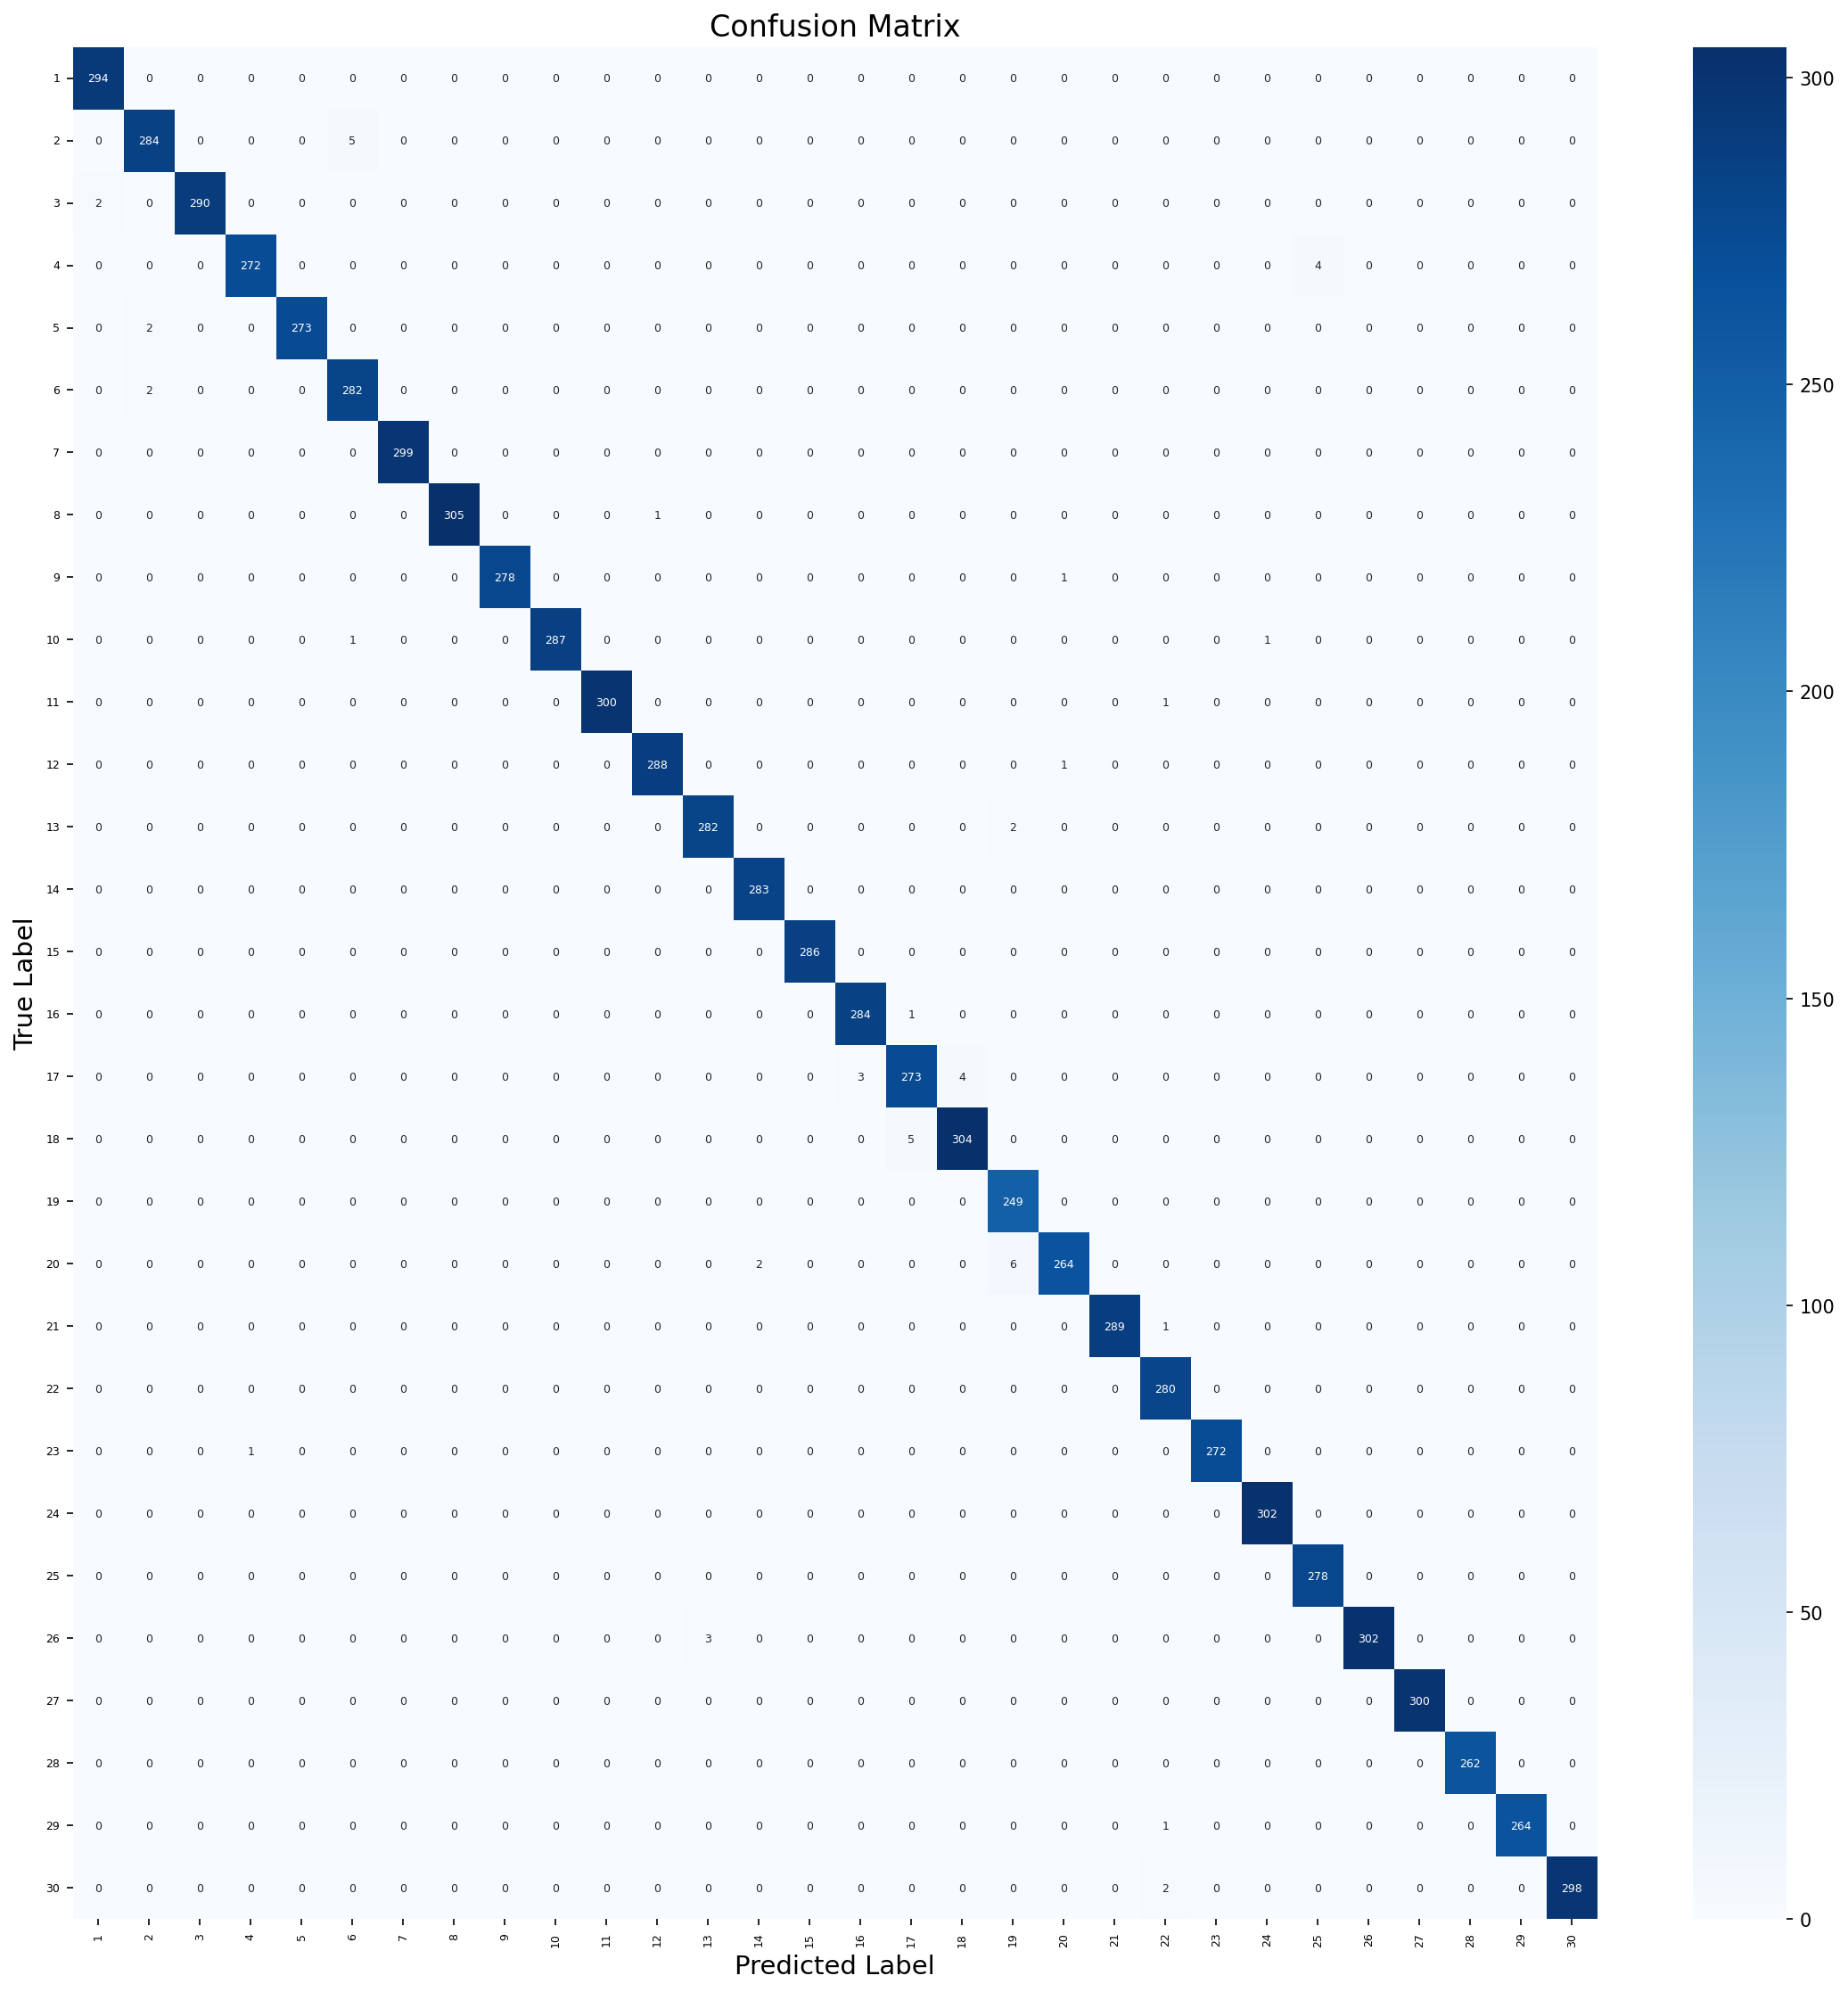
\includegraphics[width=0.5\textwidth]{figures/14nov/MobileNetV3_1D_LSTM_lr1e-04_bs8_adam_wd1e-05_ep150_confusion_matrix.png}
\caption{MobileNetV3-1D-LSTM (14 Nov): confusion matrix on the validation split.}
\label{fig:mobnet_cm_14nov}
\end{figure}

\begin{figure}[H]
\centering
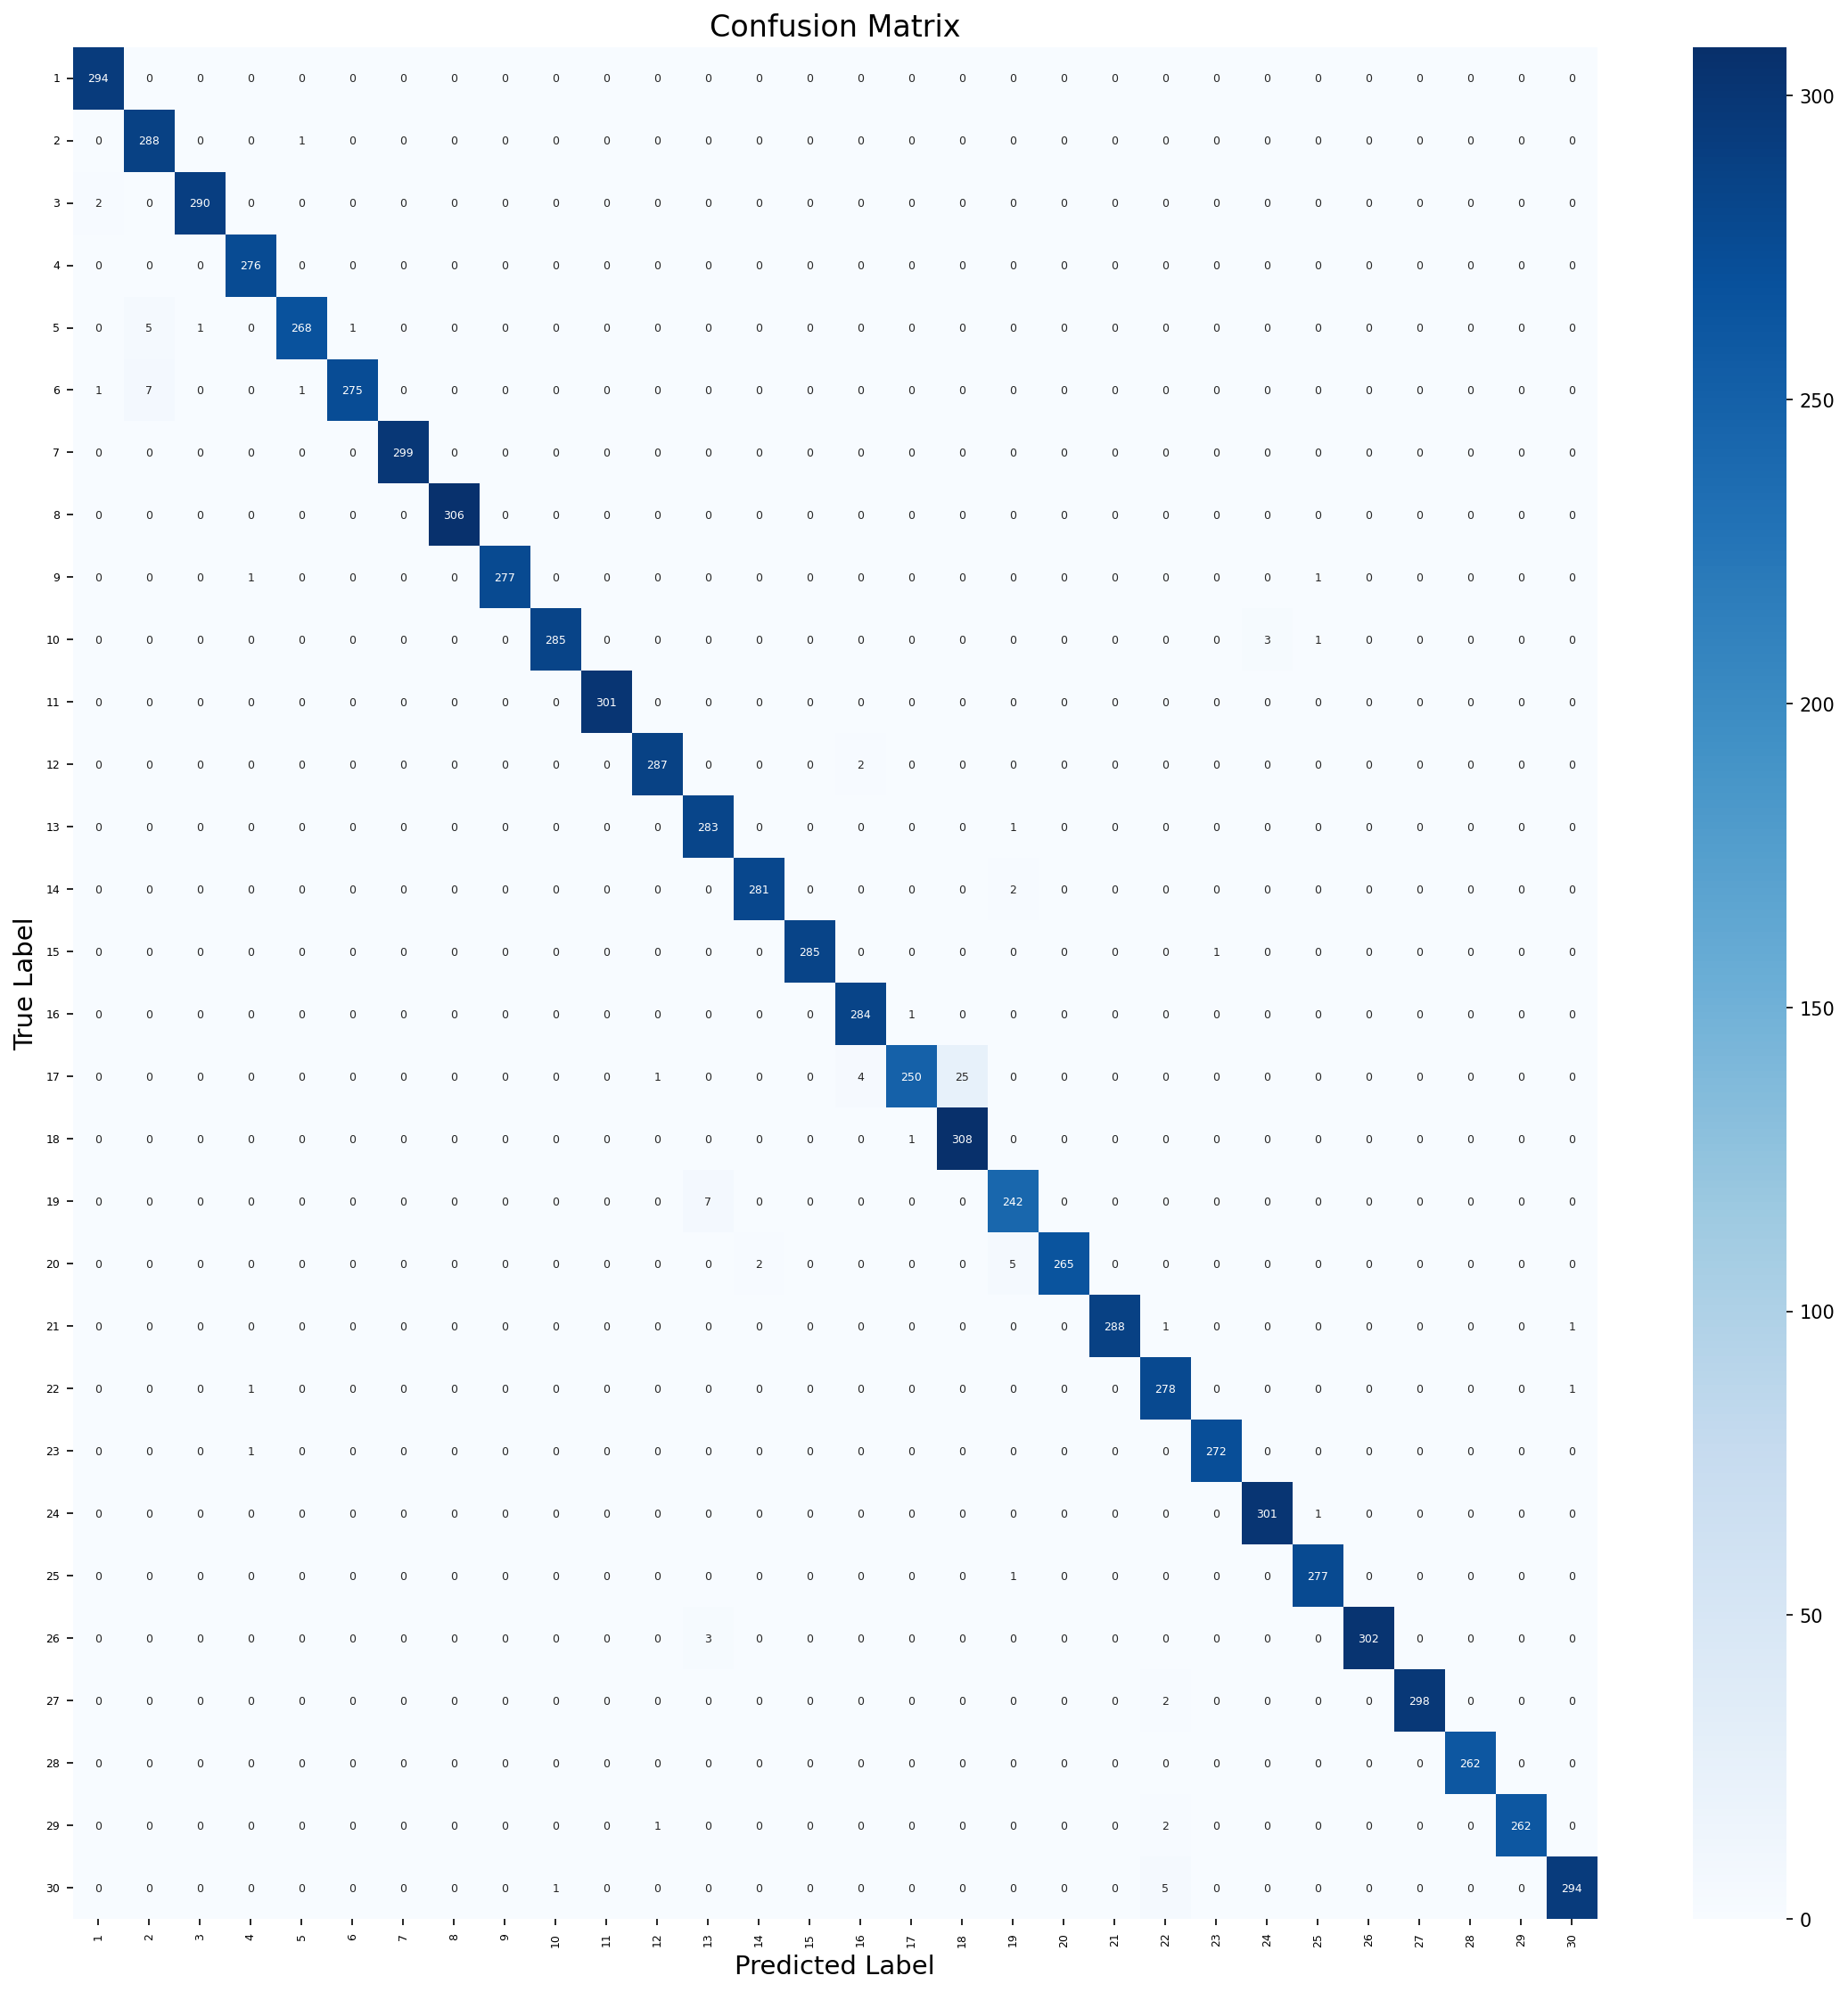
\includegraphics[width=0.5\textwidth]{figures/14nov/EfficientNet1DLSTM_lr1e-04_bs8_adam_wd1e-05_ep150_confusion_matrix.png}
\caption{EfficientNet1D-LSTM (14 Nov): confusion matrix on the validation split.}
\label{fig:efficient_cm_14nov}
\end{figure}

\begin{figure}[H]
\centering
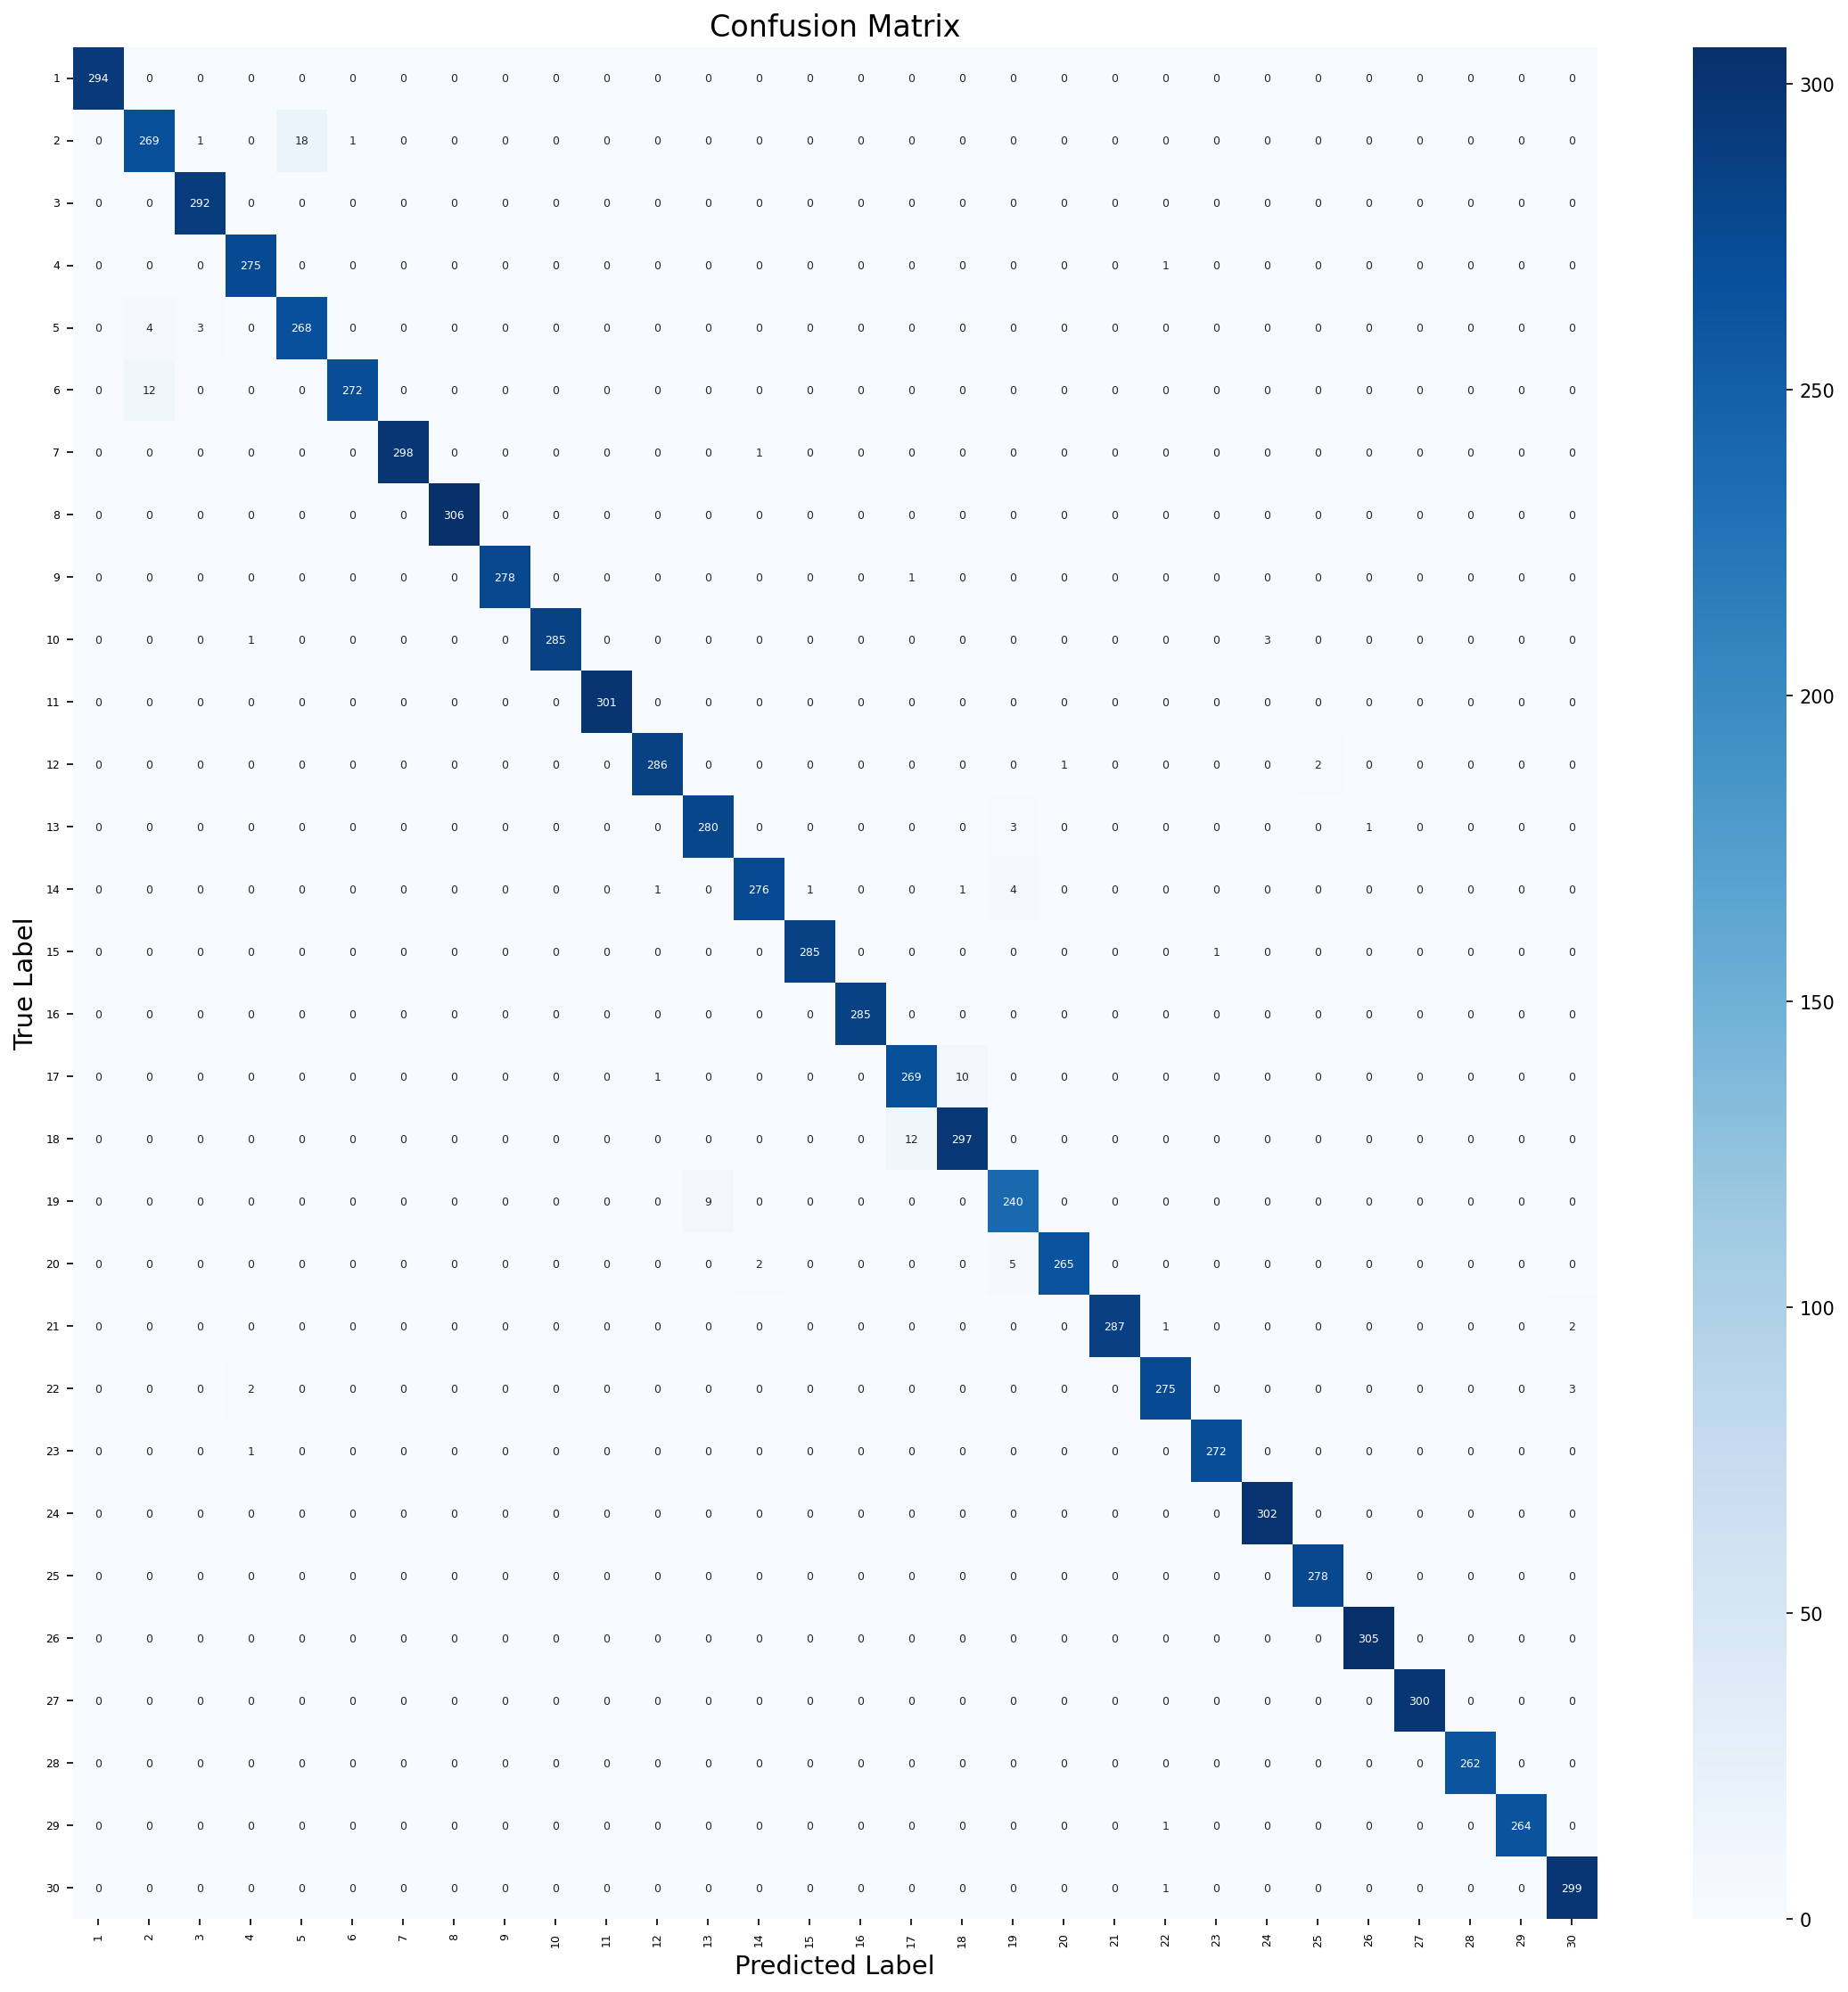
\includegraphics[width=0.5\textwidth]{figures/14nov/DenseNet1D_lr1e-04_bs8_adam_wd1e-05_ep150_confusion_matrix.png}
\caption{DenseNet1D (14 Nov): confusion matrix on the validation split.}
\label{fig:densenet_cm_14nov}
\end{figure}

These results established DenseNet1D as the most promising architecture
for further optimisation.

%==============================================================
\subsection{27 November: DenseNet Hyperparameter Optimisation}
\label{subsec:densenet_27nov}
%==============================================================

In the second phase, DenseNet1D was subjected to a dedicated
hyperparameter sweep to refine its performance.  
Four configurations were evaluated by varying learning rate and batch size:

\begin{itemize}
    \item learning rates: $1\times 10^{-4}$ and $5\times 10^{-4}$,
    \item batch sizes: $32$ and $64$,
    \item weight decay fixed at $1\times 10^{-5}$,
    \item training for 100 epochs per configuration.
\end{itemize}

\begin{table}[H]
\centering
\scriptsize
\caption{27 November --- DenseNet1D hyperparameter sweep results.}
\label{tab:densenet_hparam_sweep}
\begin{tabular}{|l|c|c|c|c|c|}
\hline
\textbf{Run} & \textbf{Batch Size} & \textbf{LR} & \textbf{WD} &
\textbf{Val Acc} & \textbf{Macro F1} \\ \hline
DenseNet1D\_lr1e-04\_bs64 & 64 & $1\times 10^{-4}$ & $1\times 10^{-5}$ &
\textbf{0.9833} & \textbf{0.9833} \\ \hline
DenseNet1D\_lr5e-04\_bs64 & 64 & $5\times 10^{-4}$ & $1\times 10^{-5}$ &
0.9805 & 0.9806 \\ \hline
DenseNet1D\_lr1e-04\_bs32 & 32 & $1\times 10^{-4}$ & $1\times 10^{-5}$ &
0.9763 & 0.9762 \\ \hline
DenseNet1D\_lr5e-04\_bs32 & 32 & $5\times 10^{-4}$ & $1\times 10^{-5}$ &
0.9762 & 0.9762 \\ \hline
\end{tabular}
\end{table}

The best-performing configuration (learning rate $1\times 10^{-4}$,
batch size $64$) achieved a validation accuracy of $98.33\,\%$ and macro
F1-score of $0.9833$.  
On the held-out test set, the same model yielded approximately
$96\,\%$ accuracy, which is adopted as the final, realistic performance
estimate for DenseNet1D in this study.

The corresponding learning curves confirm smooth convergence and minimal
overfitting. Training and validation accuracies remain within one
percentage point of each other throughout training, while validation
loss decreases steadily without oscillation (see
Figure~\ref{fig:densenet_stats_27nov}).  

\begin{figure}[H]
\centering
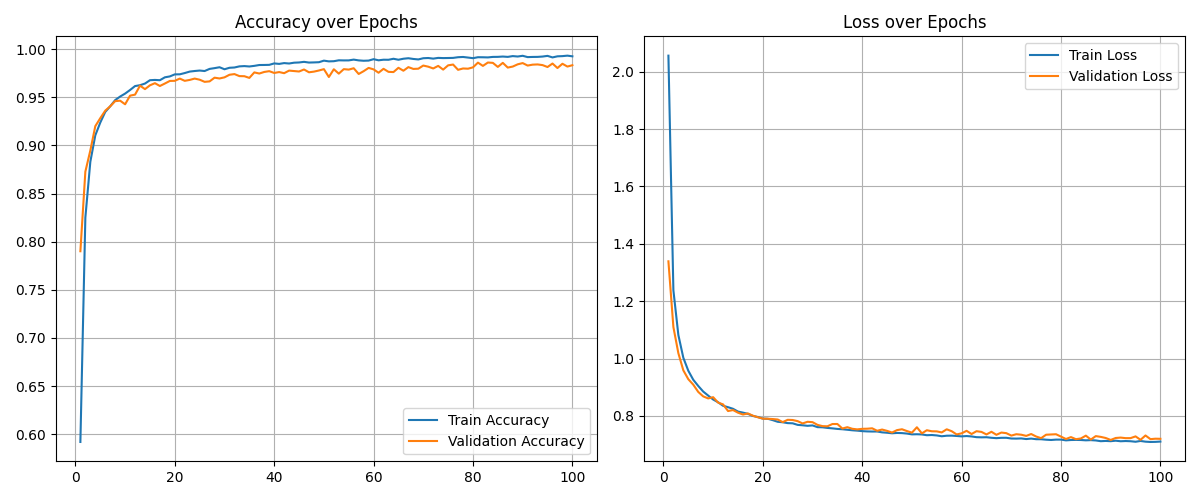
\includegraphics[width=0.9\textwidth]{figures/densenet/DenseNet1D_lr1e-04_bs64_adam_wd1e-05_ep100_stats.png}
\caption{Best DenseNet1D configuration (27 Nov): training and validation accuracy/loss.}
\label{fig:densenet_stats_27nov}
\end{figure}

Classification reports for all four DenseNet configurations on the
27 November runs show class-wise precision and recall mostly in the
range $0.97$--$1.00$, with macro and weighted averages of $0.98$--$0.99$
over 8\,576 samples. Confusion matrices (for example,
Figure~\ref{fig:densenet_cm_27nov}) display almost perfect diagonal
structure, with only a small number of isolated errors between
subjects with highly similar gait patterns.

\begin{figure}[H]
\centering
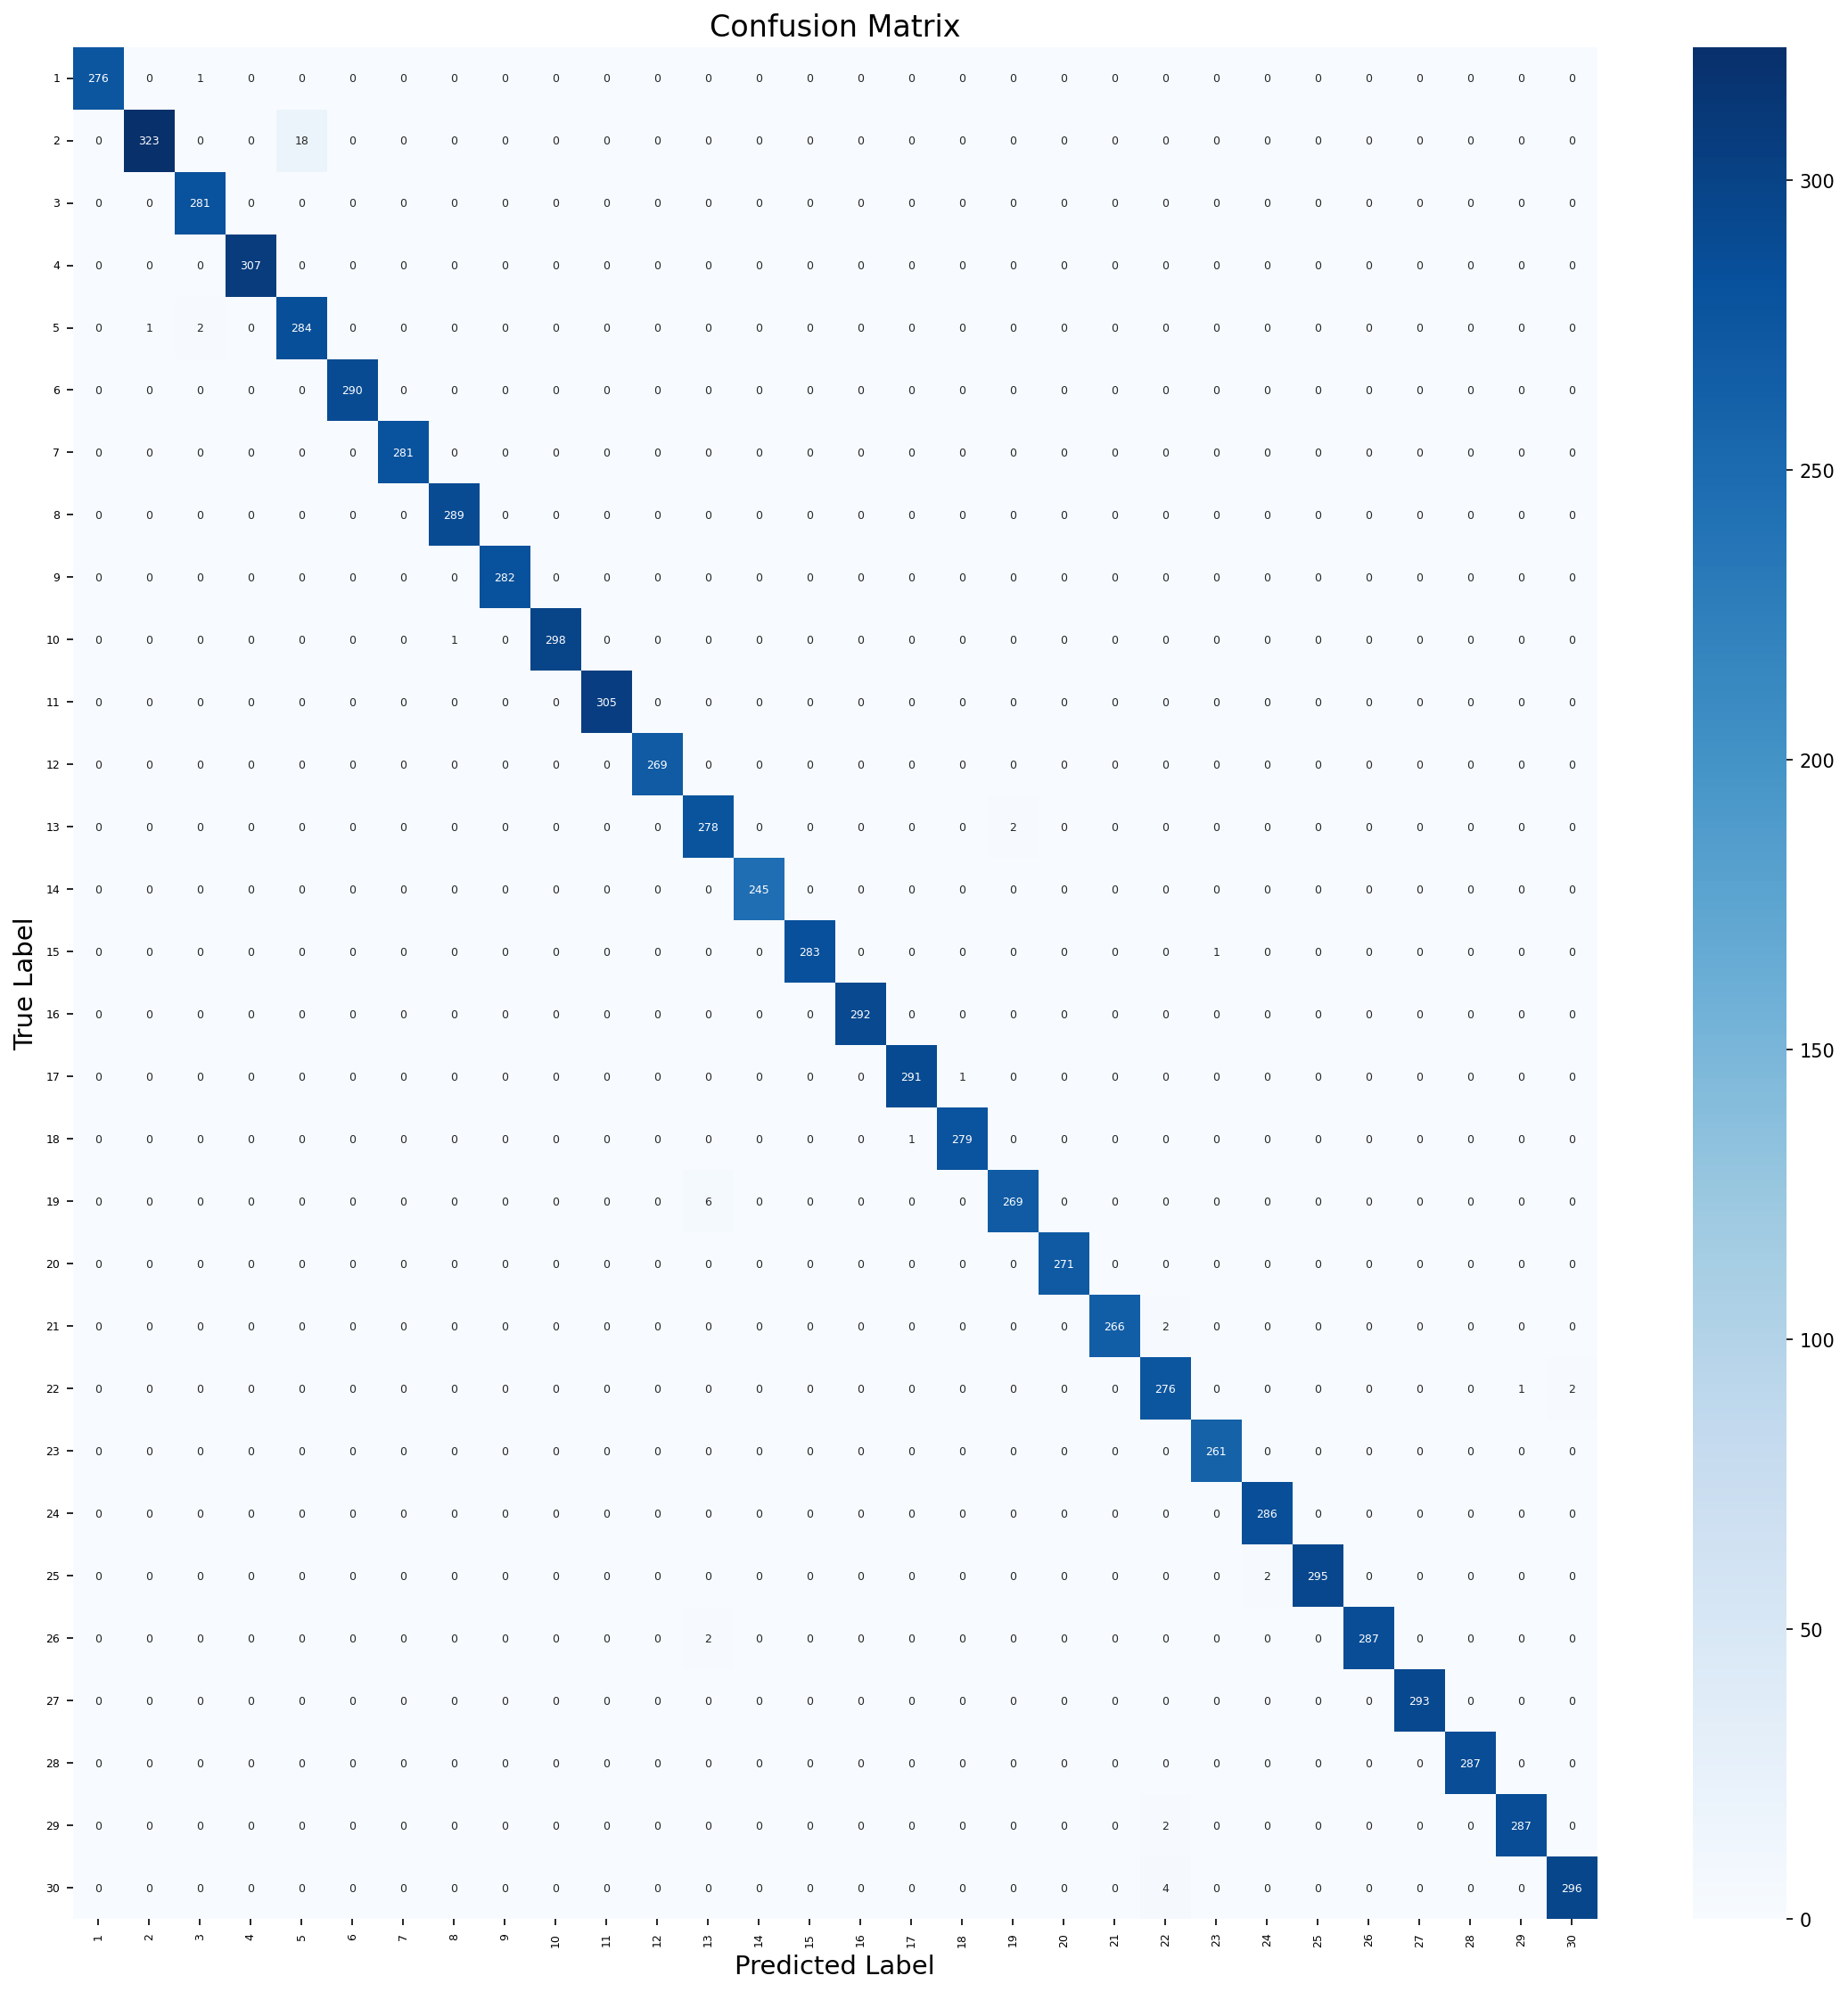
\includegraphics[width=0.7\textwidth]{figures/densenet/DenseNet1D_lr1e-04_bs64_adam_wd1e-05_ep100_confusion_matrix.png}
\caption{Confusion matrix for the best DenseNet1D model (27 Nov).}
\label{fig:densenet_cm_27nov}
\end{figure}

%==============================================================
\subsection{Combined Interpretation and Statistical Insights}
\label{subsec:combined_interpretation}
%==============================================================

Combining the 14 November and 27 November experiments yields several
clear trends:

\begin{itemize}
    \item \textbf{DenseNet1D consistently outperforms all other models.}
    It achieves the highest validation accuracy and macro F1-scores in the
    four-model comparison and further improves these metrics in the
    dedicated hyperparameter sweep.

    \item \textbf{EfficientNet1D-LSTM is a strong runner-up.}
    Its hybrid CNN--LSTM design achieves validation performance close to
    DenseNet1D and displays very stable convergence, albeit at slightly
    higher computational cost.

    \item \textbf{MobileNetV3-1D-LSTM provides an attractive
    accuracy--efficiency trade-off.}
    Although its accuracy is lower than DenseNet1D and EfficientNet1D-LSTM,
    it remains competitive and is particularly suitable for edge deployment
    scenarios.

    \item \textbf{CSILSTMNet demonstrates the limitations of LSTM-only
    models for CSI.}
    Without explicit spatial feature extraction, CSILSTMNet converges more
    slowly, exhibits higher loss variance, and obtains lower F1-scores.

    \item \textbf{DenseNet1D is robust to hyperparameter variations.}
    Across the four 27 November configurations, the standard deviation of
    validation accuracy is small ($\approx 1.3$ percentage points),
    indicating that DenseNet1D is relatively insensitive to moderate
    changes in batch size and learning rate.
\end{itemize}

Overall, the results confirm that convolutional or hybrid CNN--LSTM
architectures, and DenseNet1D in particular, are well suited for
extracting discriminative, subject-specific gait signatures from CSI
streams.

%==============================================================
\section{Discussion}
\label{sec:discussion}
%==============================================================

The experimental evidence demonstrates that deep learning models can
reliably uncover complex spatio-temporal patterns in Wi-Fi CSI that are
sufficient for robust human identification. This section interprets the
key findings and relates them to broader design and deployment
considerations.

%---------------------------------------------------------------
\subsection{Why DenseNet1D Outperforms Competing Architectures}

DenseNet1D consistently achieves the best performance due to several
architectural advantages:

\begin{itemize}
    \item \textbf{Dense connectivity.} Each layer receives inputs from all
    preceding layers, enabling strong feature reuse and improved gradient
    flow. This is especially beneficial for CSI, where relevant patterns
    can span a wide range of subcarriers and time steps.

    \item \textbf{Rich spatial feature extraction.} CSI contains structured
    patterns across subcarriers that correspond to multipath propagation
    effects. DenseNet1D's stacked 1D convolutions capture these patterns
    effectively before temporal aggregation, leading to better separation
    of subject-specific gait signatures.

    \item \textbf{Stable optimisation behaviour.} The learning curves for
    DenseNet1D show smooth convergence and very small train--validation
    gaps, indicating that the model's capacity matches the complexity of
    the data and that regularisation is effective.
\end{itemize}

These properties explain why DenseNet1D outperforms both the LSTM-only
baseline and the other hybrid CNN--LSTM models in this study.

%---------------------------------------------------------------
\subsection{Role of Hybrid CNN--LSTM Models}

EfficientNet1D-LSTM and MobileNetV3-1D-LSTM illustrate the value of
combining convolutional and recurrent layers for CSI-based
identification:

\begin{itemize}
    \item The CNN front-end extracts local spatial features and short-term
    temporal patterns.

    \item The LSTM back-end aggregates information across longer time
    horizons, capturing the sequence-level structure of gait.
\end{itemize}

EfficientNet1D-LSTM, in particular, provides near-DenseNet performance
with excellent convergence stability. MobileNetV3-1D-LSTM, while slightly
less accurate, remains attractive where computational efficiency and
energy consumption are critical, such as on embedded Wi-Fi routers.

%---------------------------------------------------------------
\subsection{Limitations of LSTM-Only Approaches}

CSILSTMNet serves as a useful baseline by highlighting the limitations
of relying solely on recurrent layers. Without convolutional preprocessing,
the LSTMs receive raw CSI sequences in which spatial correlations across
subcarriers are not explicitly modeled. This results in slower
convergence, greater sensitivity to noise, and lower overall accuracy.
The findings align with prior studies emphasising the importance of
CNN-based front-ends for RF sensing tasks \parencite{csibench2025}.

%---------------------------------------------------------------
\subsection{Impact of CSI Variability and Environmental Factors}

Occasional spikes in validation loss across several runs can be
attributed to:

\begin{itemize}
    \item dynamic multipath changes induced by other moving objects,
    \item transient interference and channel fluctuations,
    \item subtle differences in subject speed or trajectory.
\end{itemize}

DenseNet1D and EfficientNet1D-LSTM showed the strongest robustness to
such perturbations, likely because their convolutional receptive fields
can average out local fluctuations while still maintaining sensitivity
to systematic gait-induced variations.

%---------------------------------------------------------------
\subsection{Implications for Real-World Deployment}

The achieved performance (approximately 96\,\% test accuracy and
macro F1-scores close to 0.99 for DenseNet1D) indicates that Wi-Fi
CSI-based identification is a viable, privacy-preserving alternative to
camera-based biometrics. Potential application domains include:

\begin{itemize}
    \item continuous authentication in smart homes and offices,
    \item unobtrusive monitoring in healthcare environments,
    \item access control in secure indoor facilities.
\end{itemize}

At the same time, the non-contact and pervasive nature of CSI sensing
raises important ethical and privacy considerations. Deployments should
incorporate privacy-by-design principles, such as on-device processing,
data minimisation, and explicit consent where appropriate.

%---------------------------------------------------------------
\subsection{Summary}

In summary, the combined 14 November and 27 November experiments show
that:

\begin{itemize}
    \item DenseNet1D is the most suitable architecture for CSI-based
    gait identification, achieving high accuracy, strong generalisation,
    and stable training dynamics.

    \item Hybrid CNN--LSTM architectures (EfficientNet1D-LSTM and
    MobileNetV3-1D-LSTM) provide robust alternatives, particularly when a
    balance between accuracy and efficiency is required.

    \item LSTM-only models are less effective for this task, underscoring
    the importance of spatial feature extraction for CSI.

    \item The overall performance and robustness achieved in this work
    support the feasibility of deploying Wi-Fi CSI as a practical,
    privacy-preserving biometric modality in real-world environments.
\end{itemize}
